\label{MCclosure}
To verify the consistency of the analysis chain and of the corrections applied to the  correlation distributions extracted from data, a Monte Carlo closure test was setup and tried on the $\Dzero$-h analysis.

On the Monte Carlo enriched with charm and beauty quarks (LHC18a4a2$\_$fast, with GEANT3), the correlation analysis was performed both at kinematic level and at reconstructed level. At kinematic level, only acceptance cuts were applied on the D mesons and the associated particles, using the Monte Carlo information for the identification of the D mesons and the hadrons in the event and rejecting the non-primary particles. At reconstructed level, the analysis was performed as if it were executed on data, applying the event selection, the acceptance cuts for D mesons and the associated particles, selecting the D meson candidates with filtering cuts on their daughters, topological cuts and PID selection, and then keeping only the true D mesons by matching with the Monte Carlo truth; non-primary particles were rejected by means of the DCA selection. Event mixing correction was applied both at reconstructed and at kinematic level, where it takes into account just the effects of the acceptance cuts. In addition, at reconstructed level, the efficiency corrections for D mesons and associated tracks were also applied.

Examples of correlation plots at both steps are shown in Figures ~\ref{fig:MC_Kine} and~\ref{fig:MC_Reco}, separating the correlation contribution of associated tracks and D mesons from different origins, as described in the legend of the plots.

\clearpage
\begin{figure}
{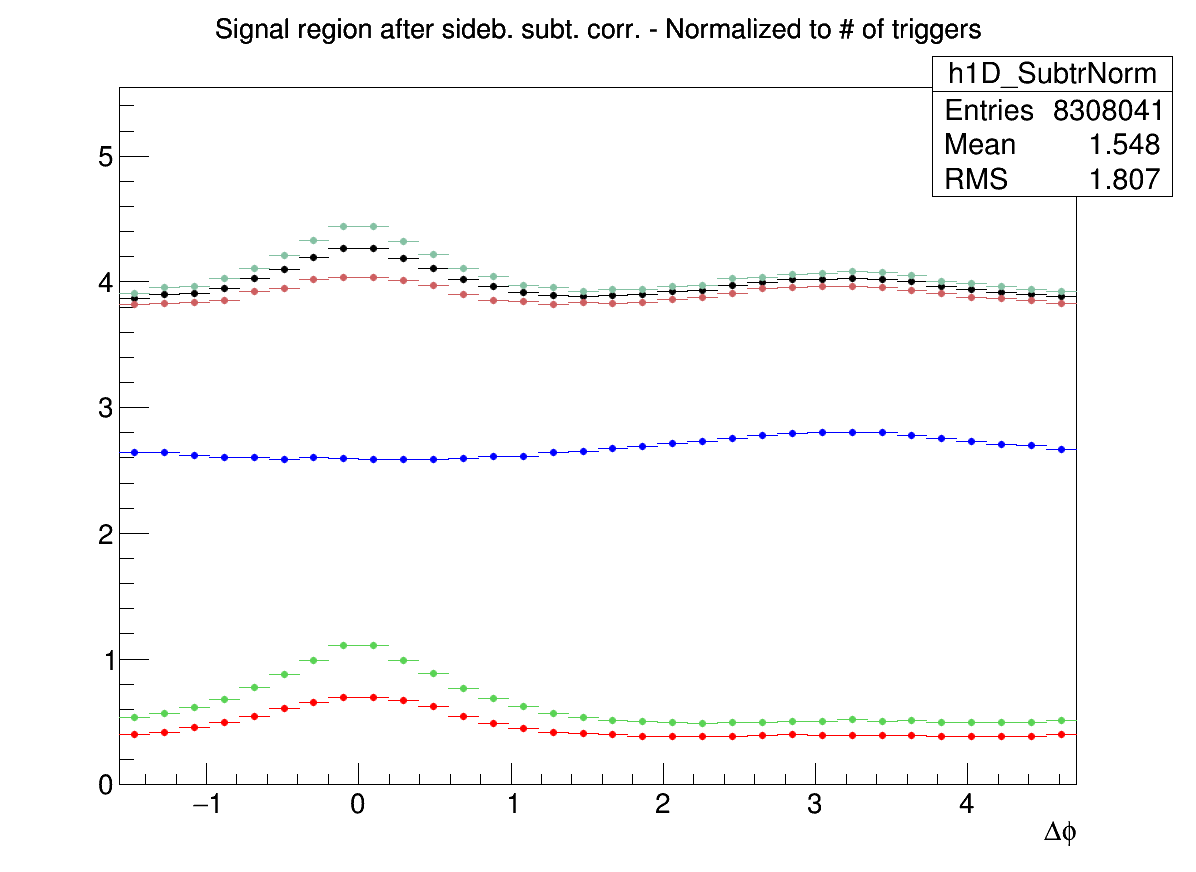
\includegraphics[width=.48\linewidth]{figures/MC_closure/AzimCorrDistr_Dzero_Canvas_PtIntBins4to5_PoolInt_thr03to1_Superimposed_Kine.png}}
{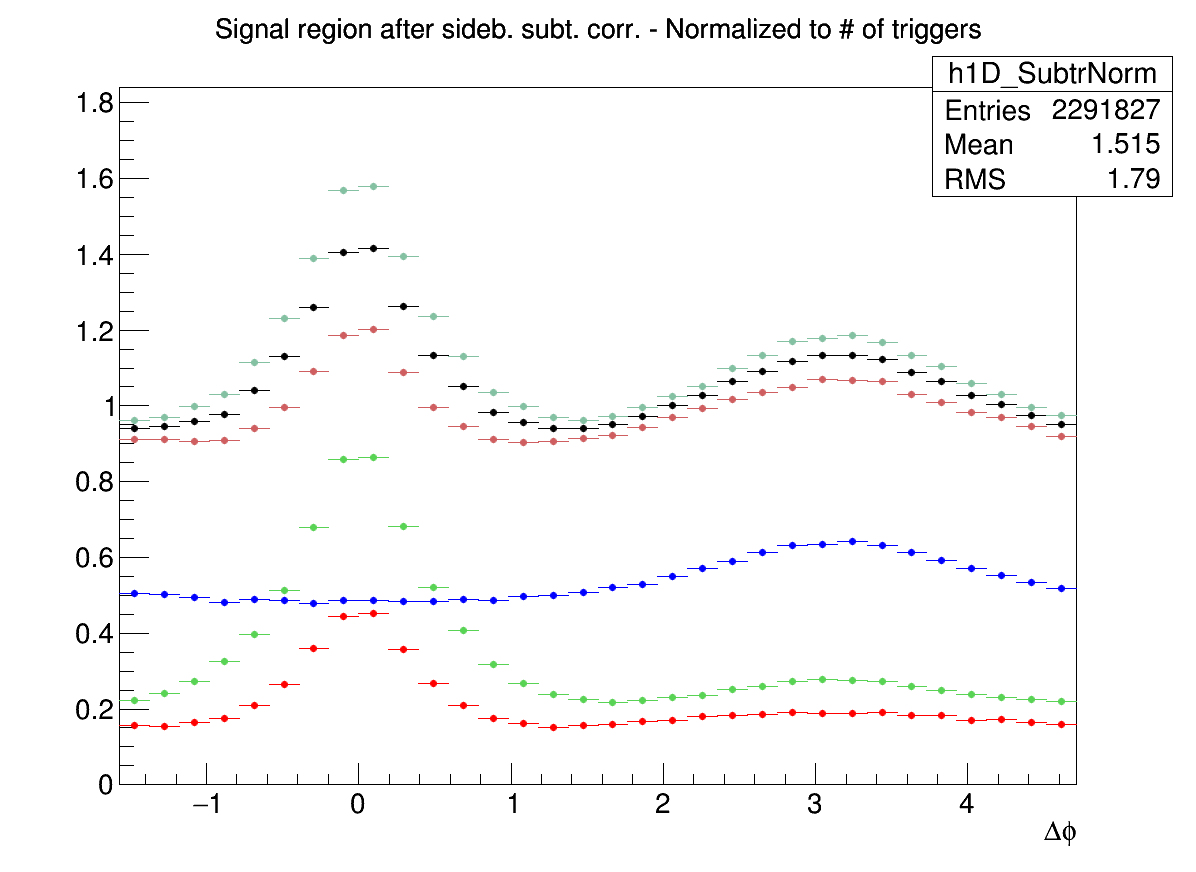
\includegraphics[width=.48\linewidth]{figures/MC_closure/AzimCorrDistr_Dzero_Canvas_PtIntBins4to5_PoolInt_thr1to99_Superimposed_Kine.png}} \\
{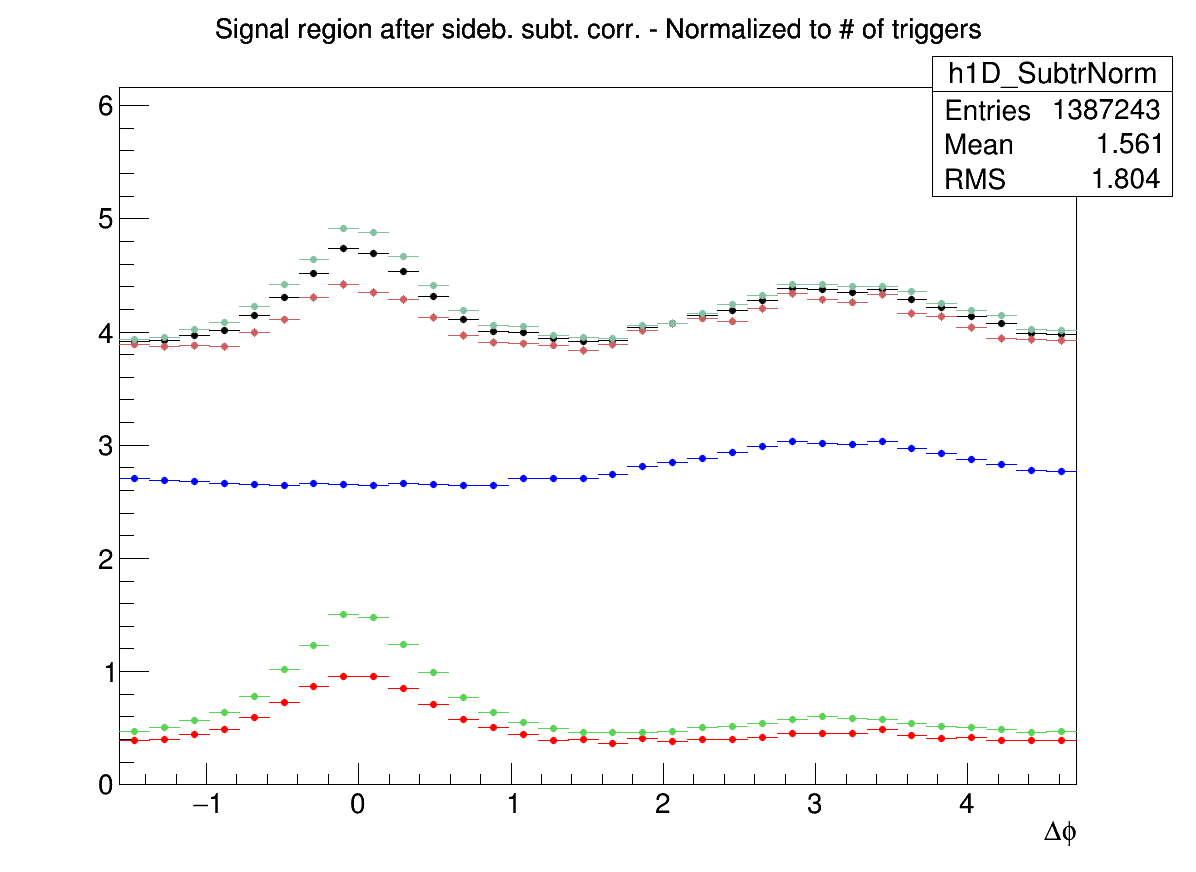
\includegraphics[width=.48\linewidth]{figures/MC_closure/AzimCorrDistr_Dzero_Canvas_PtIntBins9to10_PoolInt_thr03to1_Superimposed_Kine.png}}
{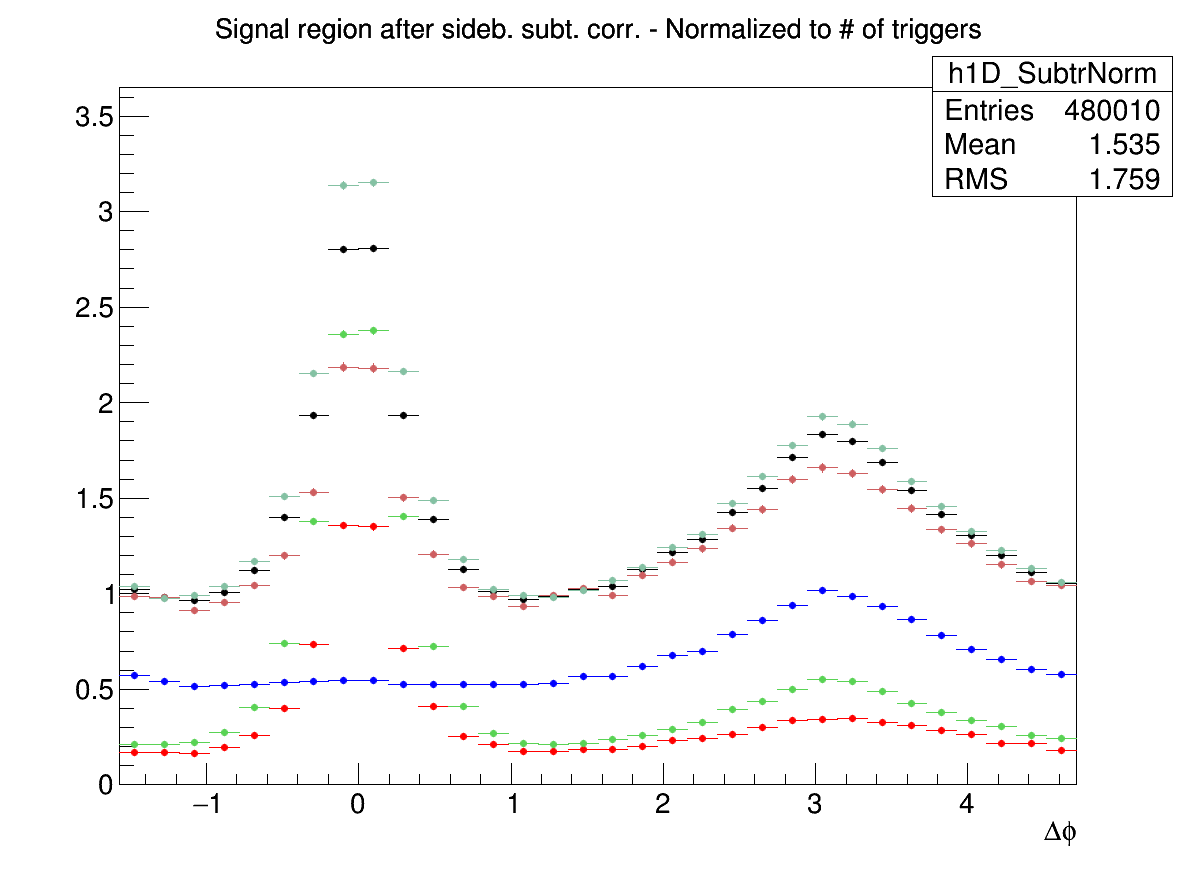
\includegraphics[width=.48\linewidth]{figures/MC_closure/AzimCorrDistr_Dzero_Canvas_PtIntBins9to10_PoolInt_thr1to99_Superimposed_Kine.png}}
\caption{$\Dzero$-hadrons azimuthal correlation distribution obtained from Monte Carlo, at kinematic step. Black points: All $\Dzero$-all hadrons, normalized by all $\Dzero$ triggers; light red points: $\Dzero$ from c-hadrons from c, normalized by c-$\Dzero$ triggers; dark red points: $\Dzero$ from c-all hadrons, normalized by c-$\Dzero$ triggers; light green points: $\Dzero$ from b-hadrons from b, normalized by b-$\Dzero$ triggers; dark green points: $\Dzero$ from b-all hadrons, normalized by b-$\Dzero$ triggers; blue points: All $\Dzero$-hadrons from light quarks, normalized by all $\Dzero$ triggers.
The panels show the ranges: $3 < \pt$(D)$ < 5$ $\gev/c$ , $0.3 < \pt$(assoc)$ < 1$ $\gev/c$  (top-left); $3 < \pt$(D)$ < 5$ $\gev/c$ , $\pt$(assoc)$ > 1$ $\gev/c$  (top-right); $8 < \pt$(D)$ < 16$ $\gev/c$ , $0.3 < \pt$(assoc)$ < 1$ $\gev/c$  (bottom-left); $8 < \pt$(D)$ < 16$ $\gev/c$ , $\pt$(assoc)$ > 1$ $\gev/c$  (bottom-right).}
\label{fig:MC_Kine}
\end{figure}

\begin{figure}
{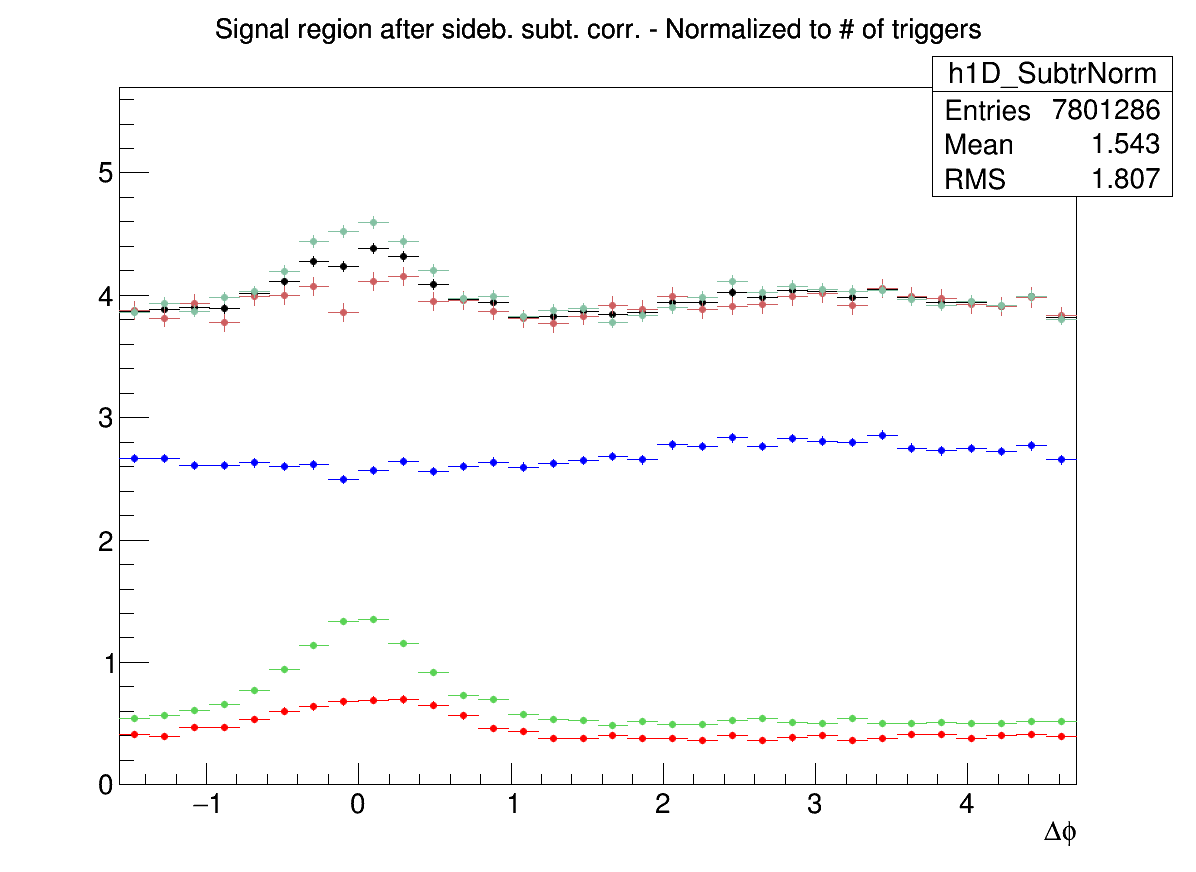
\includegraphics[width=.48\linewidth]{figures/MC_closure/AzimCorrDistr_Dzero_Canvas_PtIntBins4to5_PoolInt_thr03to1_Superimposed_Reco.png}}
{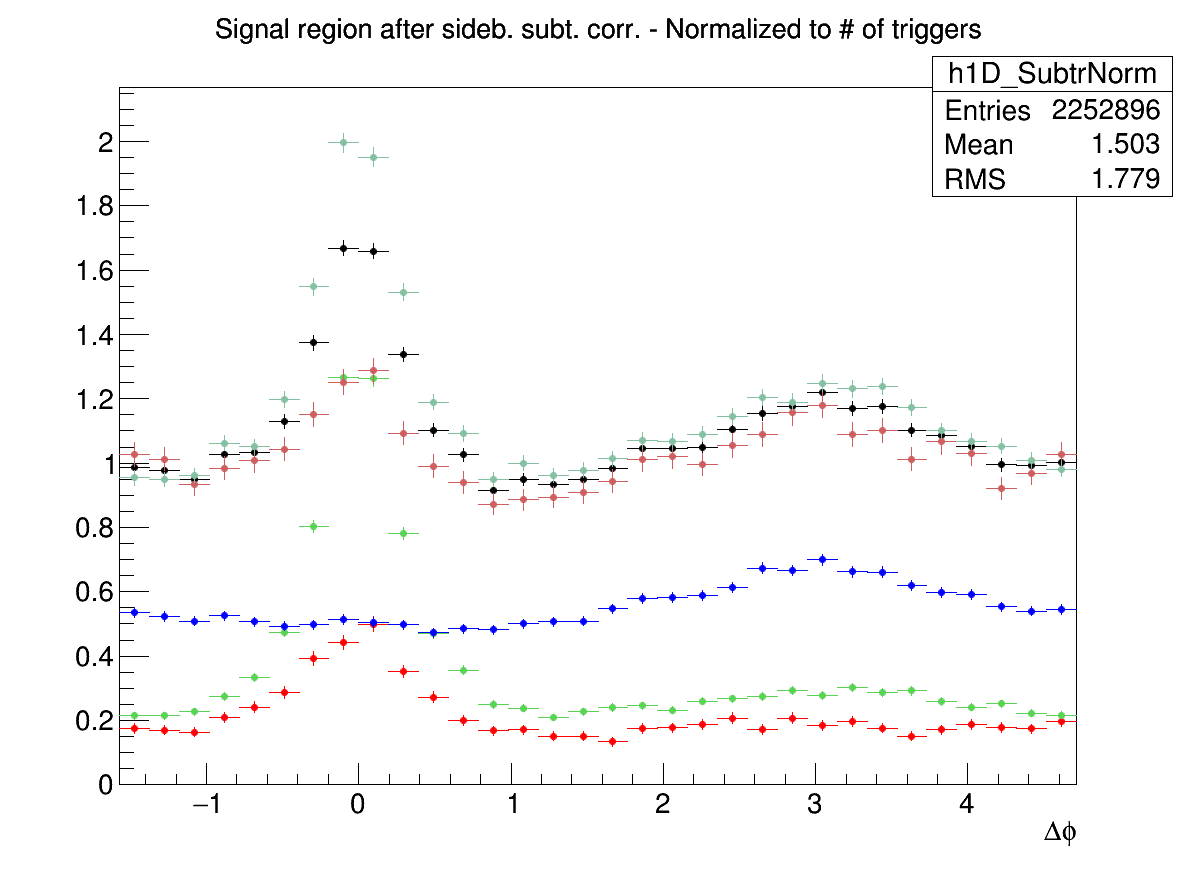
\includegraphics[width=.48\linewidth]{figures/MC_closure/AzimCorrDistr_Dzero_Canvas_PtIntBins4to5_PoolInt_thr1to99_Superimposed_Reco.png}} \\
{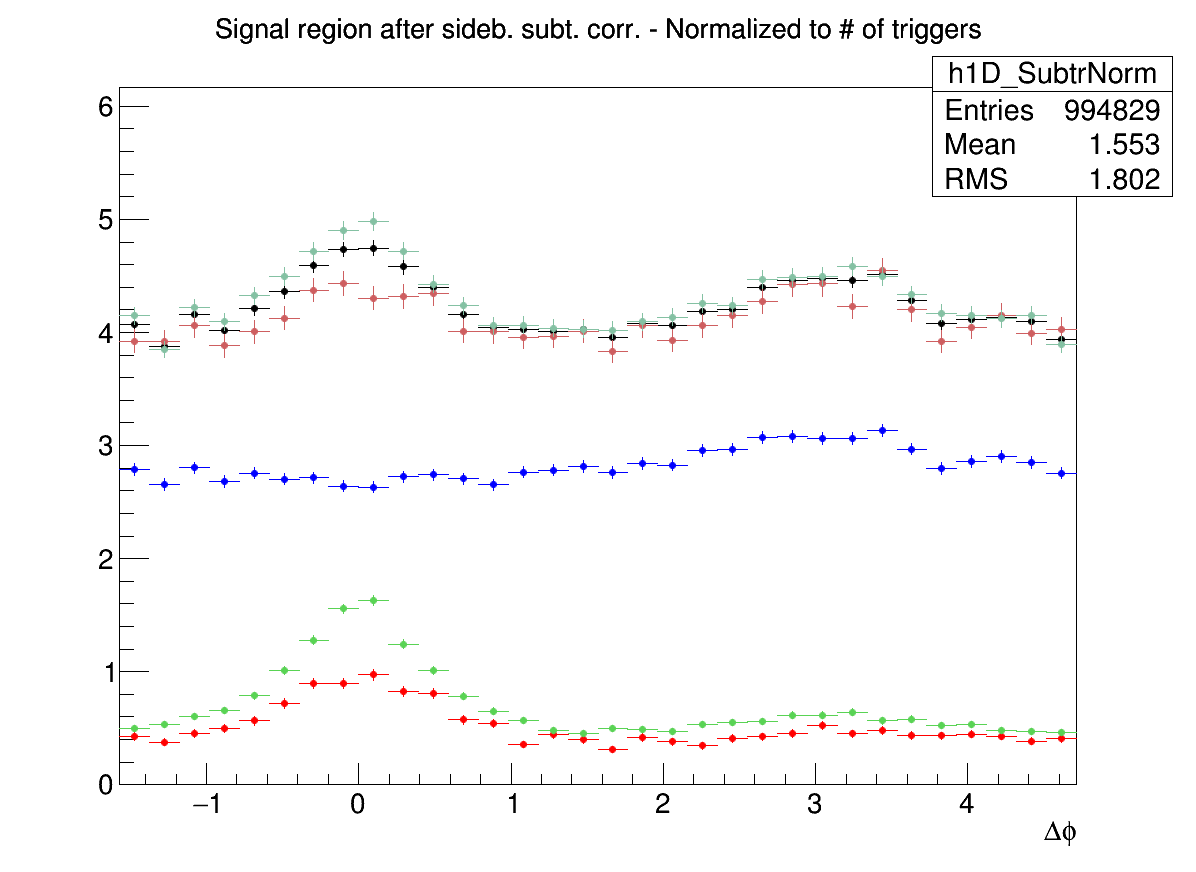
\includegraphics[width=.48\linewidth]{figures/MC_closure/AzimCorrDistr_Dzero_Canvas_PtIntBins9to10_PoolInt_thr03to1_Superimposed_Reco.png}}
{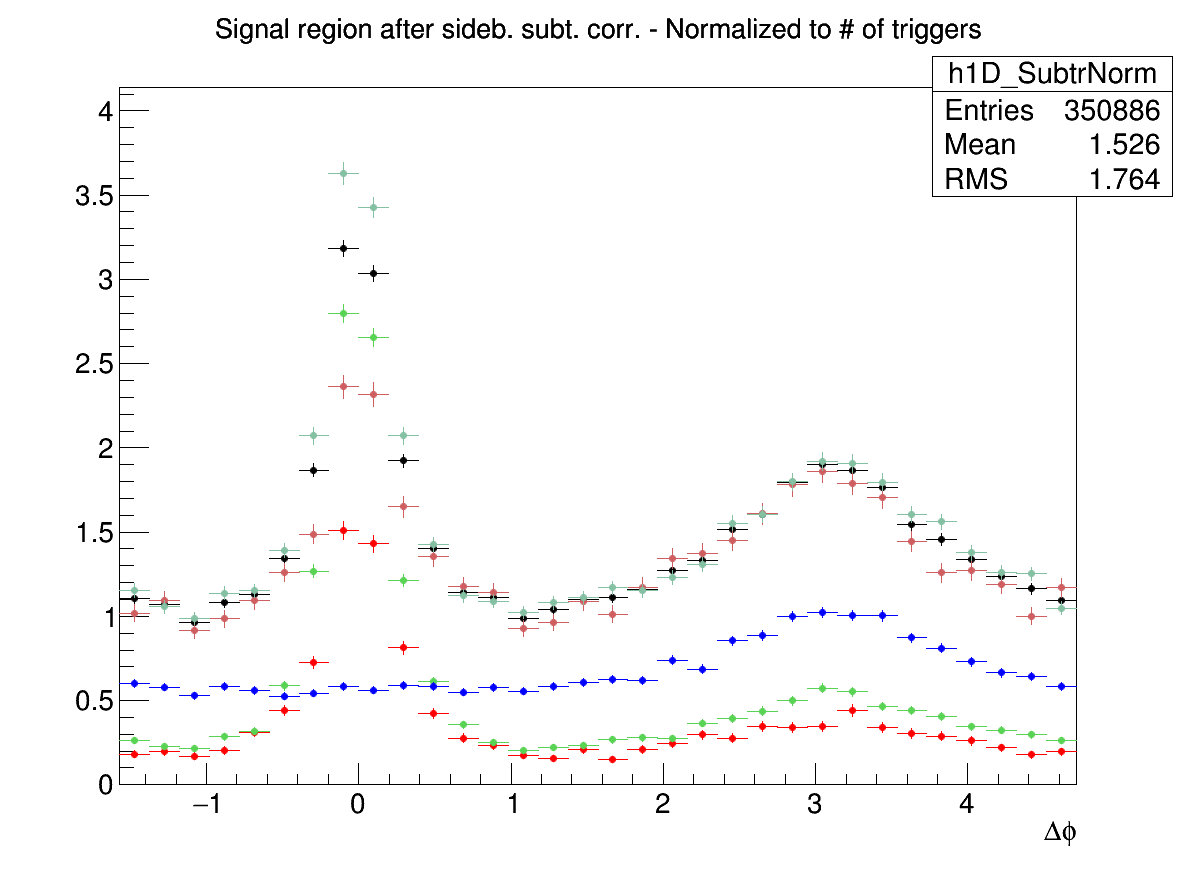
\includegraphics[width=.48\linewidth]{figures/MC_closure/AzimCorrDistr_Dzero_Canvas_PtIntBins9to10_PoolInt_thr1to99_Superimposed_Reco.png}}
\caption{$\Dzero$-hadrons azimuthal correlation distribution obtained from Monte Carlo, at reconstructed step. Black points: All $\Dzero$-all hadrons, normalized by all $\Dzero$ triggers; light red points: $\Dzero$ from c-hadrons from c, normalized by c-$\Dzero$ triggers; dark red points: $\Dzero$ from c-all hadrons, normalized by c-$\Dzero$ triggers; light green points: $\Dzero$ from b-hadrons from b, normalized by b-$\Dzero$ triggers; dark green points: $\Dzero$ from b-all hadrons, normalized by b-$\Dzero$ triggers; blue points: All $\Dzero$-hadrons from light quarks, normalized by all $\Dzero$ triggers.
The panels show the ranges: $3 < \pt$(D)$ < 5$ $\gev/c$ , $0.3 < \pt$(assoc)$ < 1$ $\gev/c$  (top-left); $3 < \pt$(D)$ < 5$ $\gev/c$ , $\pt$(assoc)$ > 1$ $\gev/c$  (top-right); $8 < \pt$(D)$ < 16$ $\gev/c$ , $0.3 < \pt$(assoc)$ < 1$ $\gev/c$  (bottom-left); $8 < \pt$(D)$ < 16$ $\gev/c$ , $\pt$(assoc)$ > 1$ $\gev/c$  (bottom-right).}
\label{fig:MC_Reco}
\end{figure}

The consistency check was performed to verify whether, after having applied all the corrections to the azimuthal correlation plots at reconstructed level, the results were compatible with the ones at kinematic level. Hence, the ratios of fully corrected reconstructed plots over kinematic plots were evaluated in all the $\Dzero$ $p_\text{T}$ bins and for the various $p_\text{T}$ thresholds for the associated tracks, separating the contributions for the different origins of particles and triggers. The ratios, shown in Figure~\ref{fig:MC_Ratios}, denote a good compatibility with 1, within the uncertainties, with the only exception being due to some structures in the near side region for the beauty origin case.
It was verified that these structures are induced by our topological selection for the D mesons. Indeed, in cases in which the D meson triggers come from B hadrons, applying the topological cuts (especially the cosine of the pointing angle) tends to favour cases with a small angular opening between the products of the B hadron decay (i.e. the D meson trigger itself and other particles), with respect to cases where the B decay particles are less collinear.

\begin{figure}
\centering
{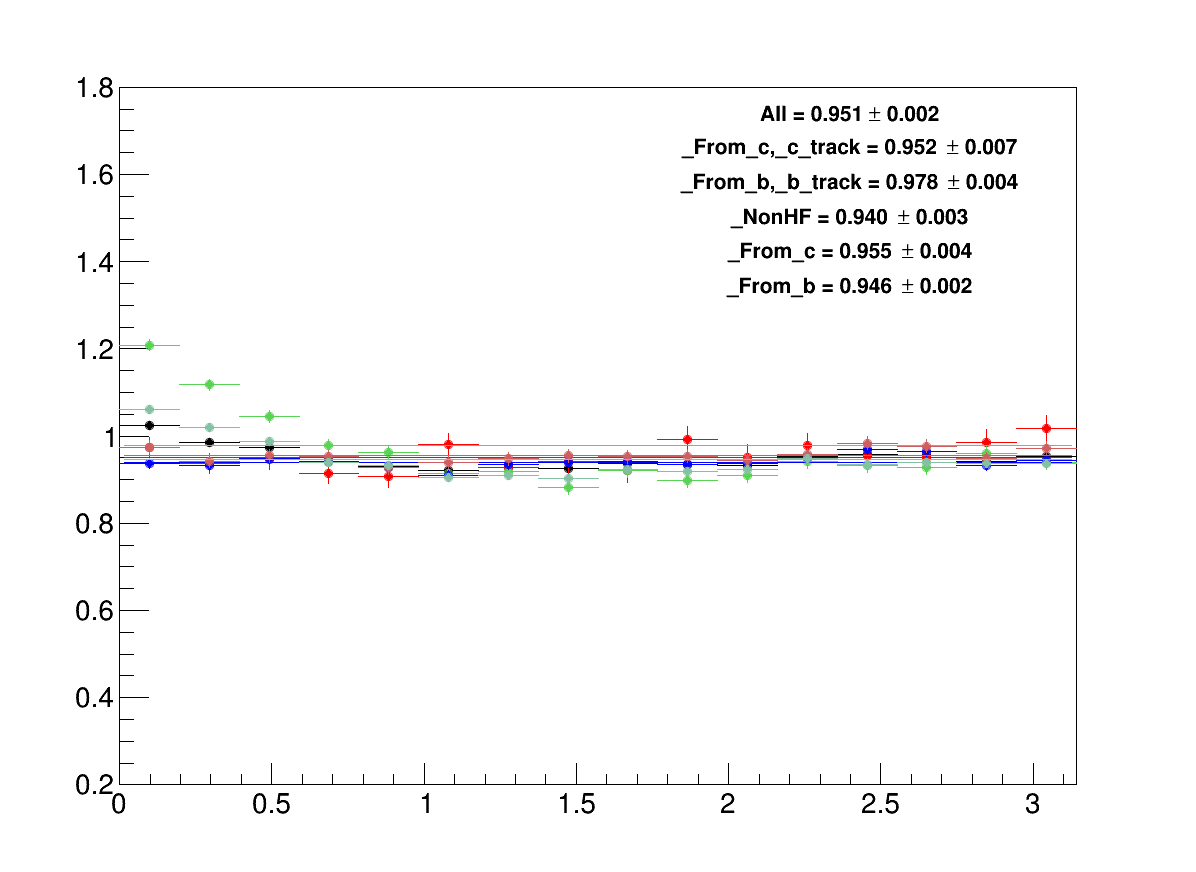
\includegraphics[width=.48\linewidth]{figures/MC_closure/MCClosure_Dzero_Canvas_PtIntBins3to3_PoolInt_thr03to1.png}}
{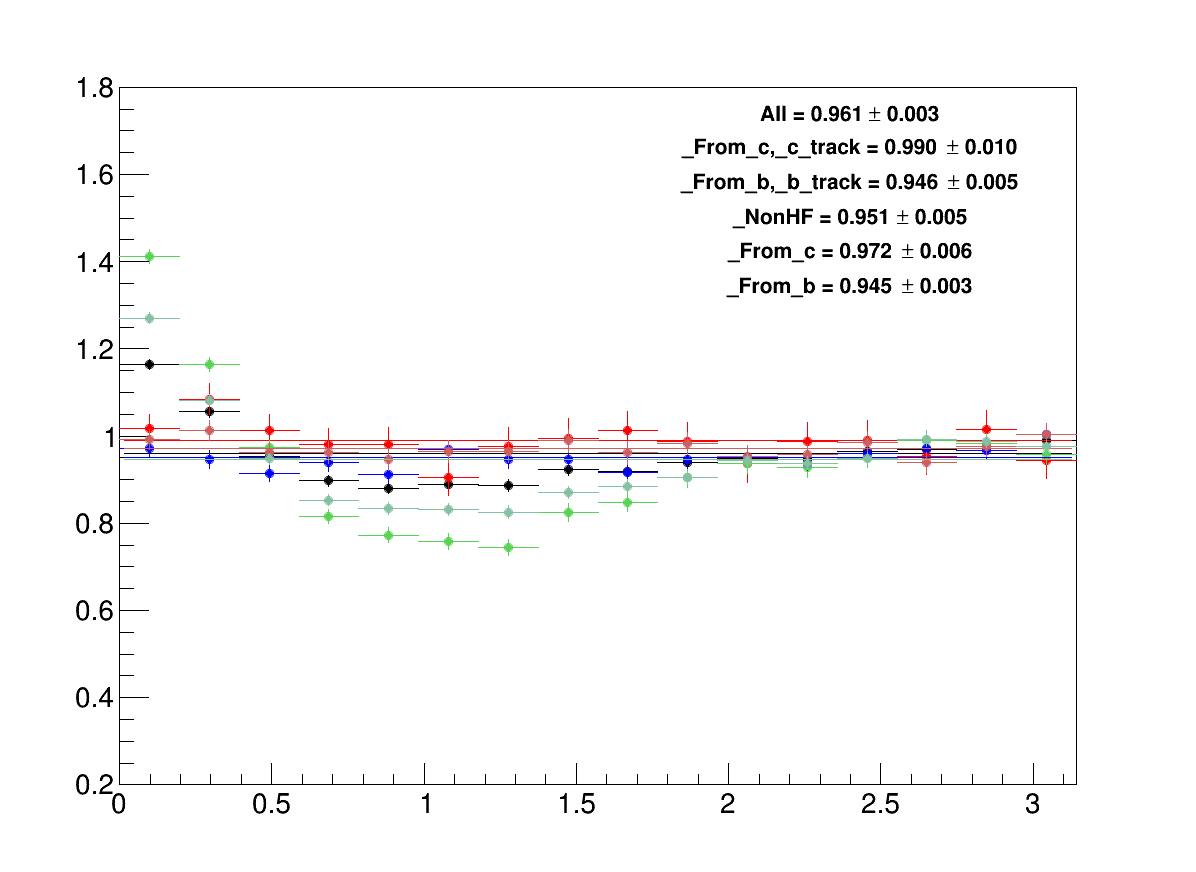
\includegraphics[width=.48\linewidth]{figures/MC_closure/MCClosure_Dzero_Canvas_PtIntBins3to3_PoolInt_thr1to99.png}} \\
{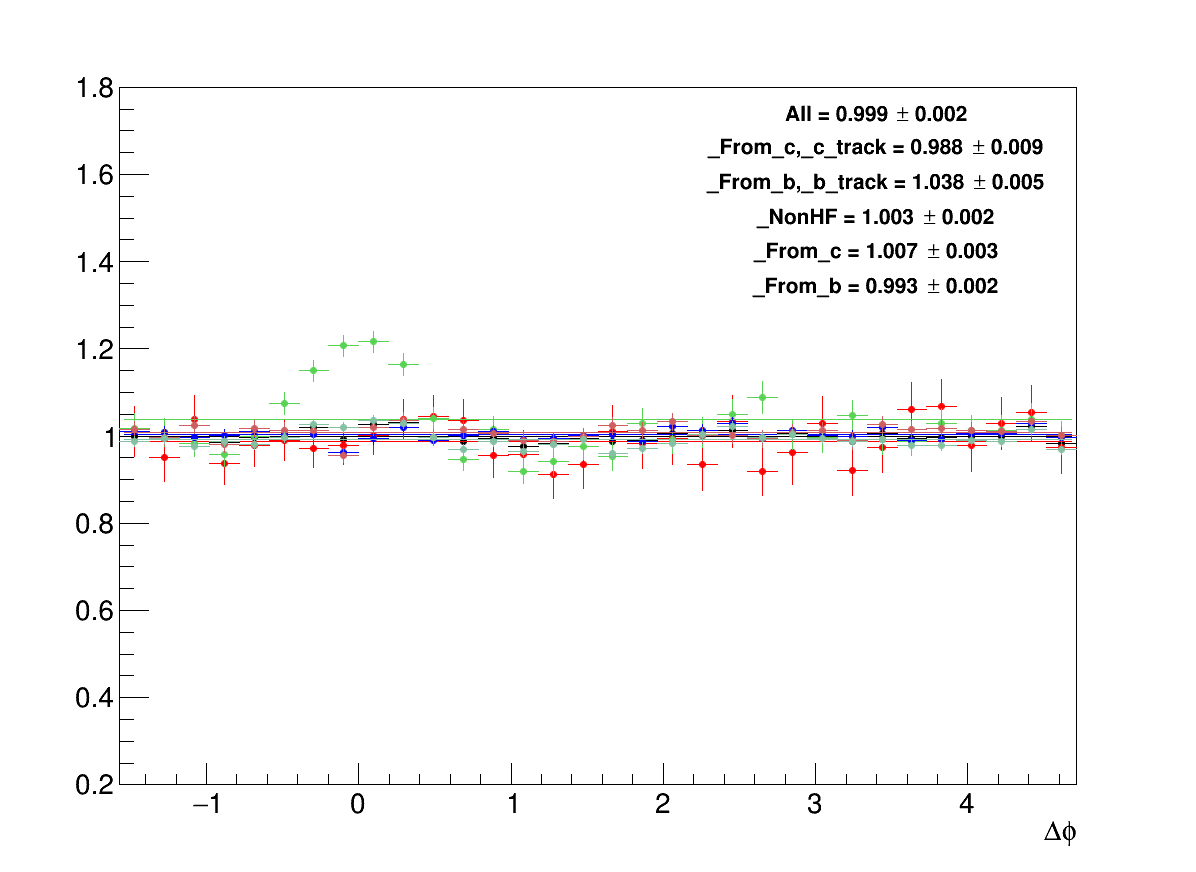
\includegraphics[width=.48\linewidth]{figures/MC_closure/MCClosure_Dzero_Canvas_PtIntBins4to5_PoolInt_thr03to1.png}}
{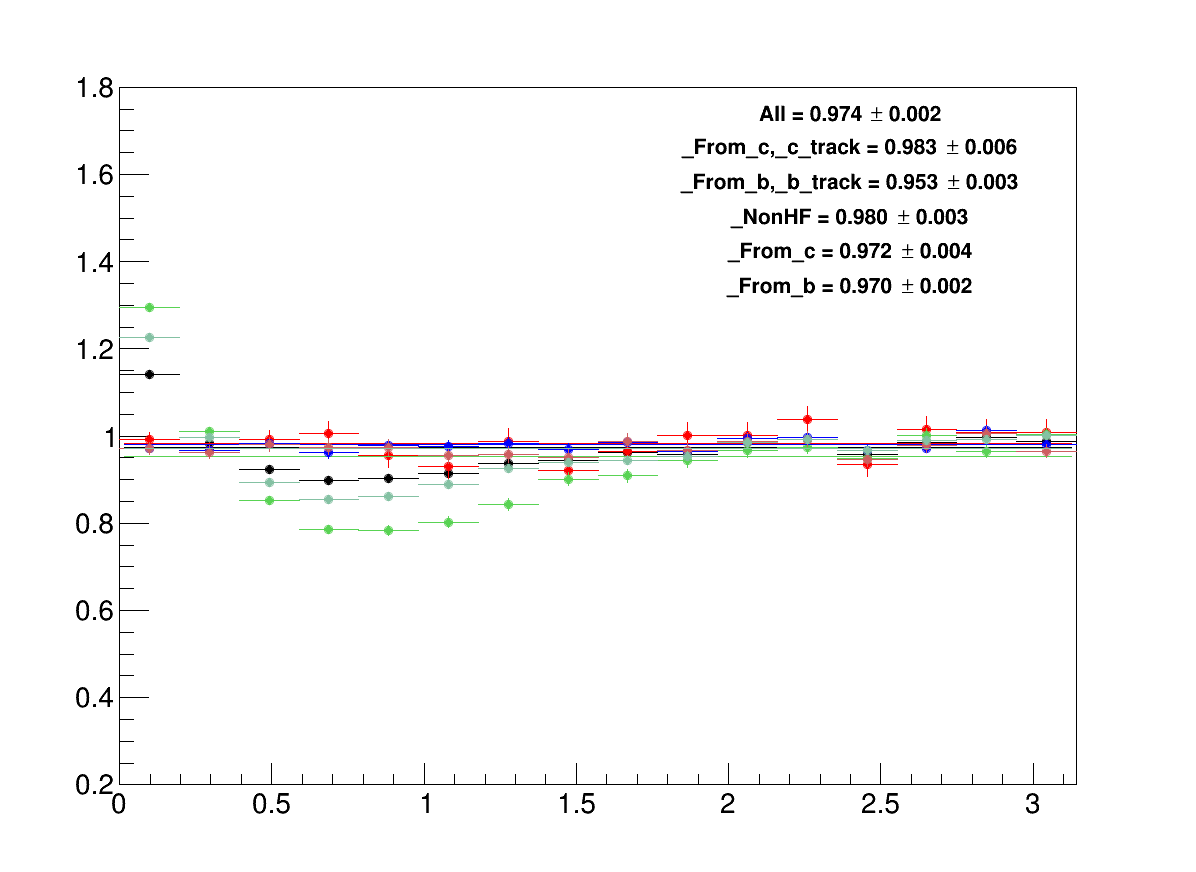
\includegraphics[width=.48\linewidth]{figures/MC_closure/MCClosure_Dzero_Canvas_PtIntBins4to5_PoolInt_thr1to99.png}} \\

{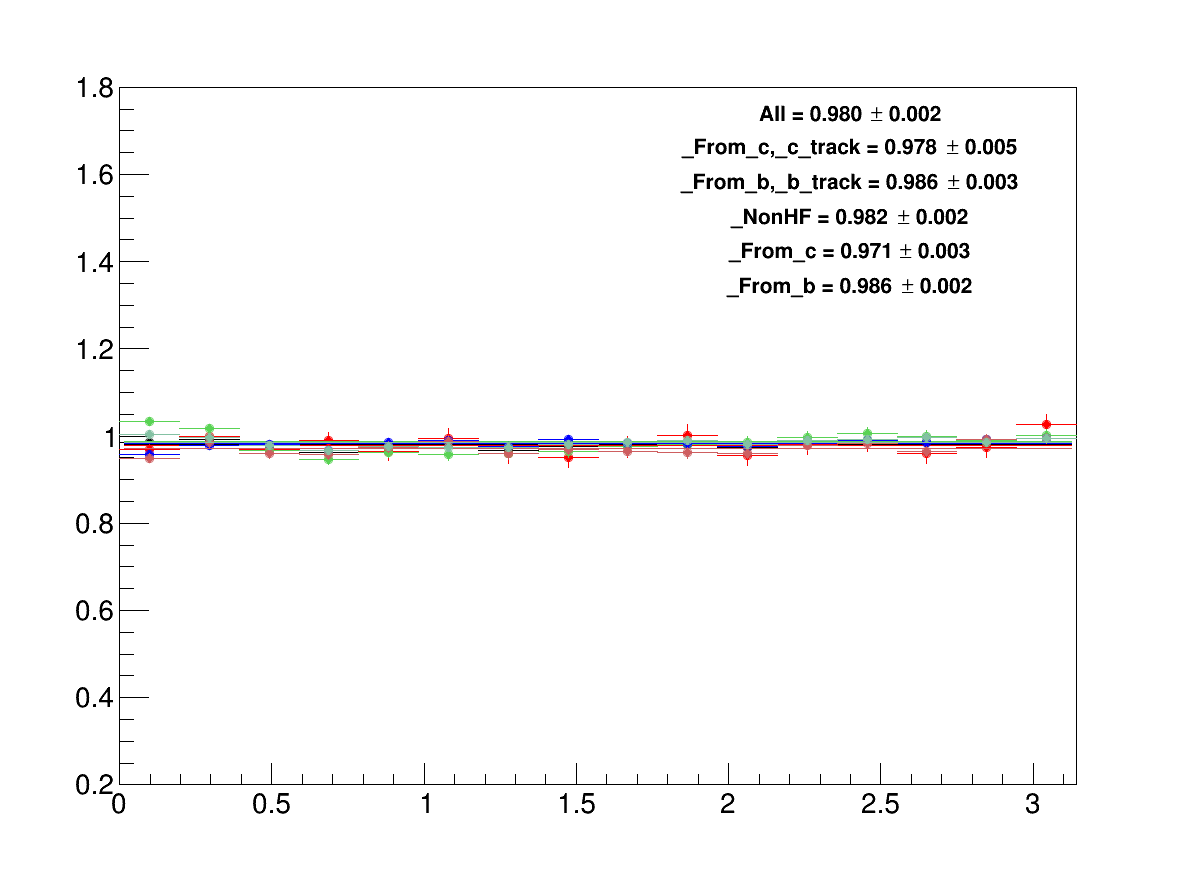
\includegraphics[width=.48\linewidth]{figures/MC_closure/MCClosure_Dzero_Canvas_PtIntBins6to8_PoolInt_thr03to1.png}}
{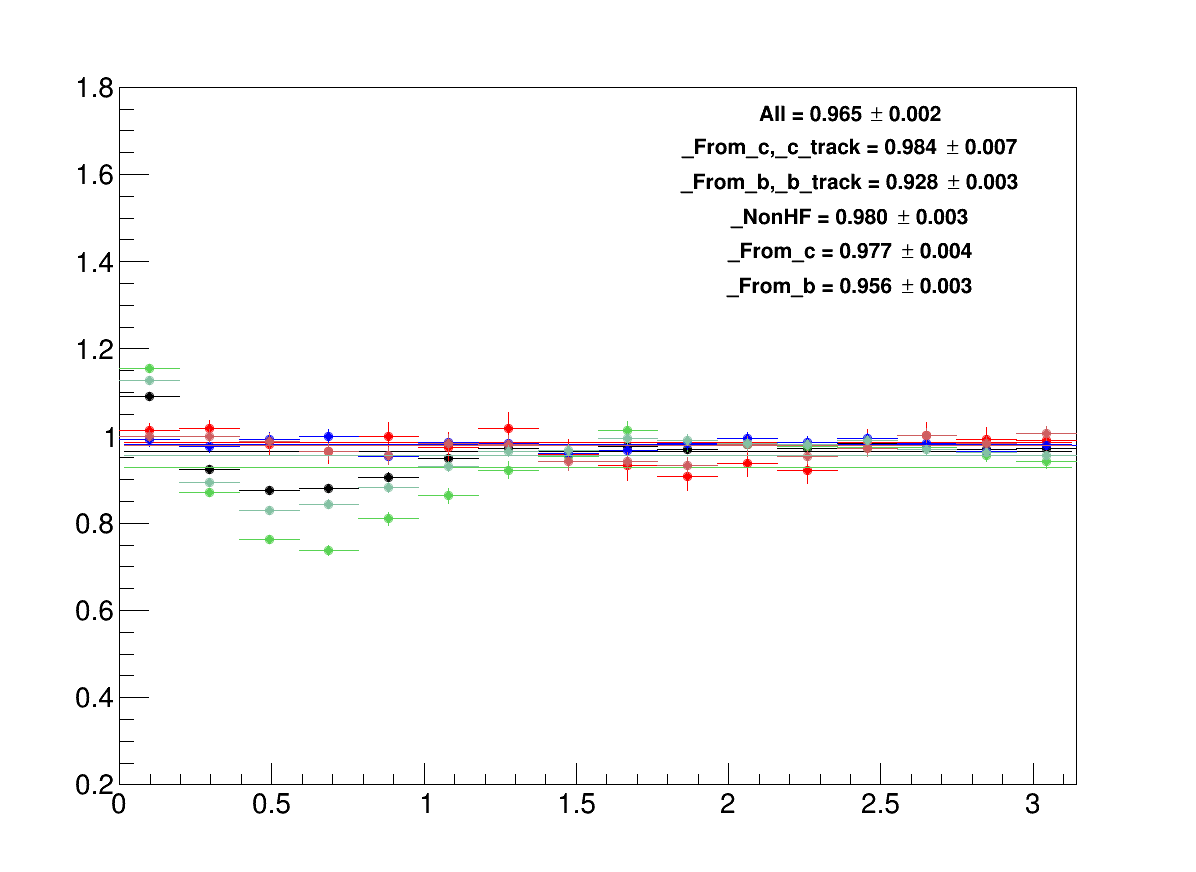
\includegraphics[width=.48\linewidth]{figures/MC_closure/MCClosure_Dzero_Canvas_PtIntBins6to8_PoolInt_thr1to99.png}} \\

{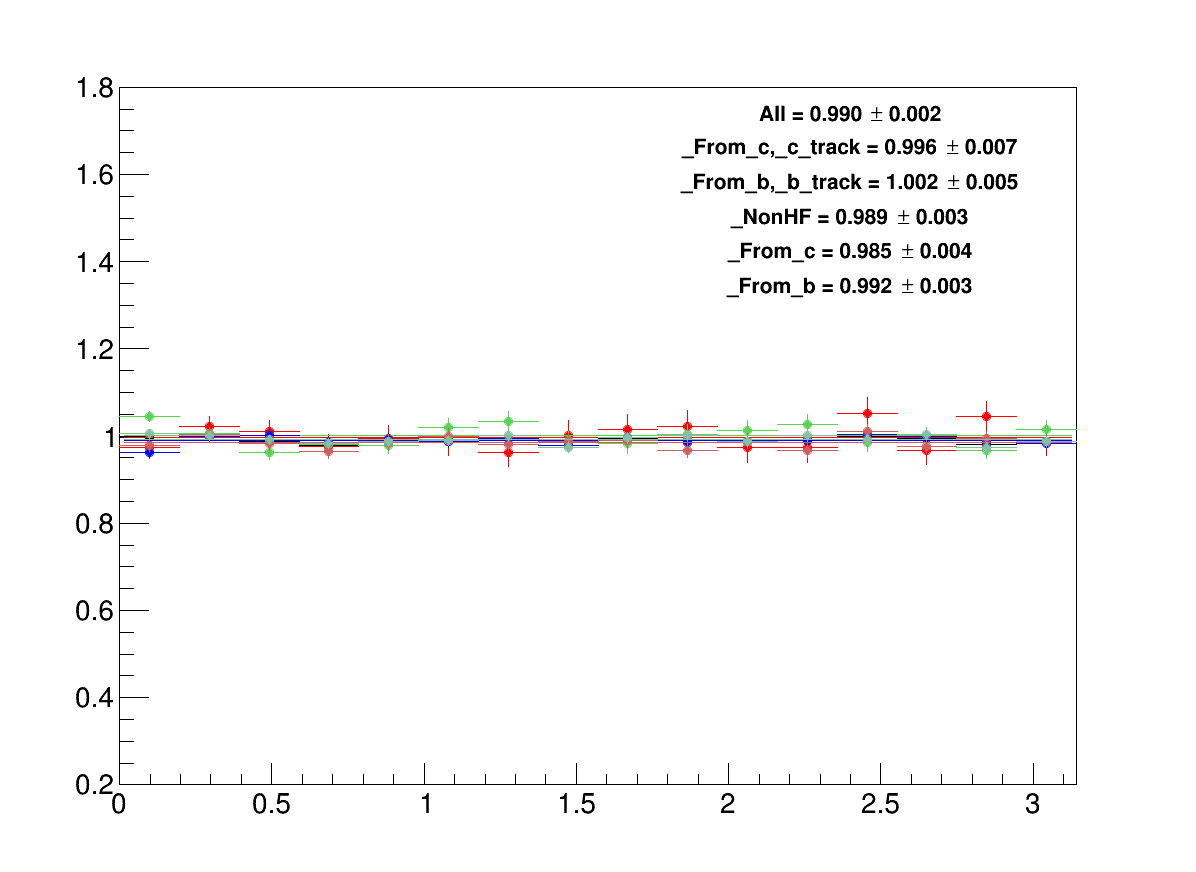
\includegraphics[width=.48\linewidth]{figures/MC_closure/MCClosure_Dzero_Canvas_PtIntBins9to11_PoolInt_thr03to1.png}}
{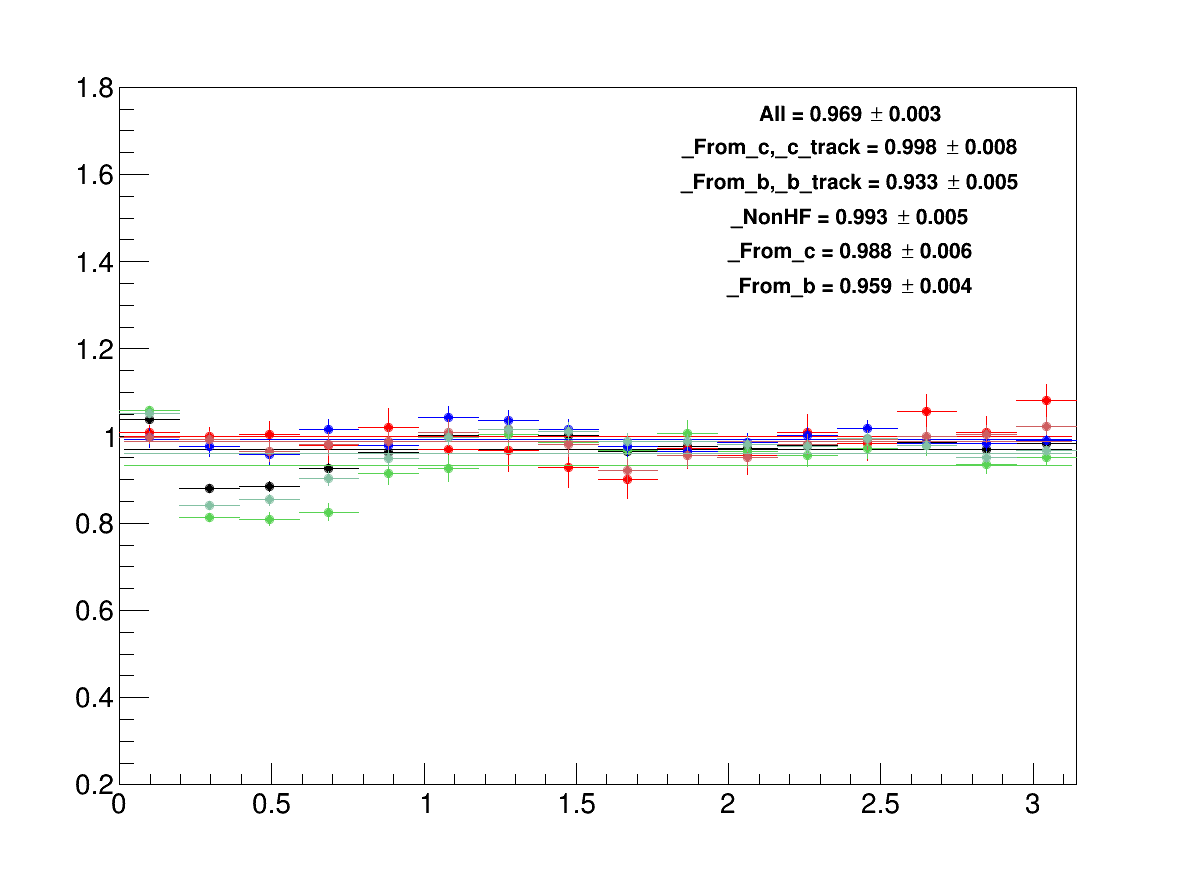
\includegraphics[width=.48\linewidth]{figures/MC_closure/MCClosure_Dzero_Canvas_PtIntBins9to11_PoolInt_thr1to99.png}}
\end{figure}
\begin{figure}
\centering
\caption{Ratios of fully corrected azimuthal correlation plots at reconstructed level over azimuthal correlation plots at kinematic level, in the two $\Dzero$ $p_\text{T}$ bins, for the different associated $p_\text{T}$ ranges. Black points: All $\Dzero$-all hadrons, normalized by all $\Dzero$ triggers; light red points: $\Dzero$ from c-hadrons from c, normalized by c-$\Dzero$ triggers; dark red points: $\Dzero$ from c-all hadrons, normalized by c-$\Dzero$ triggers; light green points: $\Dzero$ from b-hadrons from b, normalized by b-$\Dzero$ triggers; dark green points: $\Dzero$ from b-all hadrons, normalized by b-$\Dzero$ triggers; blue points: All $\Dzero$-hadrons from light quarks, normalized by all $\Dzero$ triggers.
The panels show the ranges: $2 < \pt$(D)$ < 3$ $\gev/c$ , $0.3 < \pt$(assoc)$ < 1$ $\gev/c$  (1st row-left); $2 < \pt$(D)$ < 3$ $\gev/c$ , $\pt$(assoc)$ > 1$ $\gev/c$  (1st row-right); $3 < \pt$(D)$ < 5$ $\gev/c$ , $0.3 < \pt$(assoc)$ < 1$ $\gev/c$  (2nd row-left); $3 < \pt$(D)$ < 5$ $\gev/c$ , $\pt$(assoc)$ > 1$ $\gev/c$  (2nd row-right);  $5 < \pt$(D)$ < 8$ $\gev/c$ , $0.3 < \pt$(assoc)$ < 1$ $\gev/c$  (3rd row-left), $5 < \pt$(D)$ < 8$ $\gev/c$ , $\pt$(assoc)$ > 1$ $\gev/c$  (3rd row-right); $8 < \pt$(D)$ < 16$ $\gev/c$ , $0.3 < \pt$(assoc)$ < 1$ $\gev/c$  (4th row-left), $8 < \pt$(D)$ < 16$ $\gev/c$ , $\pt$(assoc)$ > 1$ $\gev/c$  (4th row-right).}
\label{fig:MC_Ratios}
\end{figure}

In the Monte Carlo closure test, this situation is reflected in the correlation distributions at reconstructed level, where the topological selection is applied, while it does not occur at kinematic level. Hence, in the reconstructed/kinematic ratio, the distribution would show an excess for $\Delta\varphi = 0$ (due to the favoured decays with small opening angle), which is then compensated by a depletion for larger values of $\Delta\varphi = 0$ (corresponding to B decays with larger angles, which are disfavoured).
These structures are prominent at low $\Dzero$ $p_\text{T}$, where the topological cuts are tighter, and tend to disappear at higher $\pt$, where the selections are released. They are also larger in the higher associated track $\pt$ ranges, where the fraction of B-hadron decay tracks dominate the overall correlation distributions.

The data correlation distribution need to be corrected for this bias, and in particular for the enhancement of b-origin correlation pairs at the centre of the near side region, which would influence the near-side peak features.
In order to do this, the amount of the b-origin excess is evaluated from the Reco/Kine ratio, by considering the b-$\Dzero$-all tracks case (dark green points). The excess at Reco level (affecting data) is quantified as a $\Delta\varphi$ modulation {\bf modul} for the five points an each side of the $\Delta\varphi = 0$ value (or, equivalently, on the first five points of the reflected distributions, which start from $\Delta\varphi=0$. This is done separately in each $\pt$ range.
Then, the correction is done by applying this modulation to the data correlation distributions, but taking into account that only the correlation entries from B$\rightarrow$D are affected, while the c$\rightarrow$D correlations need to be left unaltered.
In particular, it has to be considered that:
\begin{itemize}
\item On data, the B$\rightarrow$D correlation pairs are only a fraction (1-$\fprompt$) of the total.
\item The amplitude of B$\rightarrow$D$|_{\rm amplit}$ correlation pattern is different (greater) than the amplitude of the c$\rightarrow$D$|_{\rm amplit}$ correlation pattern:
\end{itemize}

Thus, the following equation is applied to get the corrected $C(\Delta\varphi)_{\rm corr}$ data points starting from the raw ones, $C(\Delta\varphi)_{\rm raw}$:
\begin{equation}
C(\Delta\varphi)_{\rm corr} = C(\Delta\varphi)_{\rm raw} \cdot [\frac{{\rm c}\rightarrow{\rm D}|_{\rm amplit}}{{\rm (B+c)}\rightarrow{\rm D}|_{\rm amplit}} \cdot f_{\rm prompt} + \frac{{\rm B}\rightarrow{\rm D}|_{\rm amplit}}{{\rm (B+c)}\rightarrow{\rm D}|_{\rm amplit}} \cdot (1-f_{\rm prompt})\cdot\frac{1}{\bf modul}]
\end{equation}
where ${\rm (B+c)}\rightarrow{\rm D}|_{\rm amplit} = {\rm c}\rightarrow{\rm D}|_{\rm amplit} \cdot f_{\rm prompt} + {\rm B}\rightarrow{\rm D}|_{\rm amplit} \cdot (1-f_{\rm prompt})$, and where the two amplitudes are evaluated from the Monte Carlo distributions of Figure \ref{fig:MC_Reco} at reconstructed level (so, including the bias), and $\fprompt$ with the procedure described in \ref{feeddown}.
Applying the {\bf modul} factor to the beauty part of the data correlation distributions brings its value back to the generated level case, effectively removing the bias.
The effect of the correction is a shift of the data points in the near-side region (in general, downward in the first and second points, the upward in the others). The maximum value of the shift is of about 5\%, at the centre of the near-side peak, for the lowest D-meson $\pt$ range ($3 < \pt < 5$ $\gev/c$ ) and the highest associated track $\pt$ range ($\pt > 3$ $\gev/c$ ). The typical values are instead of a couple of percentage points. The correction is zero in the highest D-meson $\pt$ range.
To take into account for possible inaccuracies in the definition of the modulations, or in their rescaling, a systematic uncertainty is  applied on the corrected data points, with value $|C(\Delta\varphi)_{\rm corr} - C(\Delta\varphi)_{\rm raw}|/\sqrt(12)$, on each side of the data points affected by the bias (symmetric uncertainty).
 
\clearpage
%\end{document}
